\chapter{\label{a5-extractors}Charge Extractor Investigations}

\minitoc

\section{Introduction}

In Chapter~\ref{ch6-reduction}, the different algorithms for extracting charge from a waveform are extensively discussed, as well as the important considerations one must be vigilant of when producing a charge-extraction algorithm. The purpose of this appendix is to demonstrate the performance of the \textit{Cross Correlation} charge-extraction method, in contrast to the simpler \textit{Window Integration} approach. I performed this investigation in the context of the \gls{chec-s} prototype.

\section{Integration Window}

\begin{figure}
  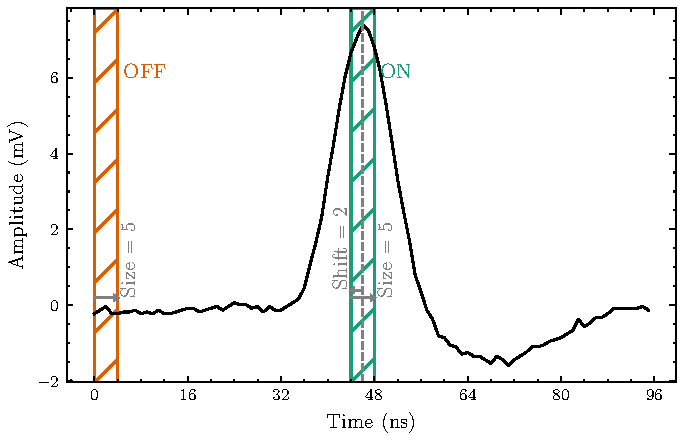
\includegraphics[width=\textwidth]{charge_extraction_window_wf}
  \caption[Definition of integration window on a waveform.]{Example waveform from a Monte Carlo simulation of CHEC-S, containing an approximately \SI{50}{\pe} signal. The ``on'' and ``off'' regions used to extract the signal-to-noise are illustrated. The window start position is defined as the peak position subtracted by the window shift. The window end position is defined as the window start plus the window size. A window size of 5 corresponds to 5 samples being included in the integration.}
  \label{fig:charge_extraction_window_wf}
\end{figure}

\begin{figure}
  \begin{subfigure}[b]{0.49\textwidth}
    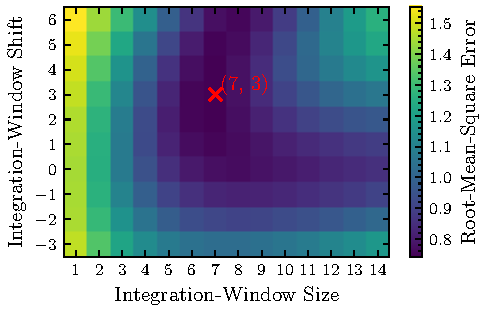
\includegraphics[width=\textwidth]{amp1nsb5}
    \caption{1~p.e. illumination, 5~MHz noise.}
    \label{fig:amp1nsb5}
  \end{subfigure}
  \hfill
  \begin{subfigure}[b]{0.49\textwidth}
    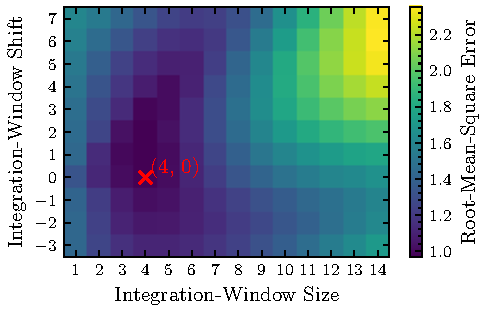
\includegraphics[width=\textwidth]{amp1nsb125}
    \caption{1~p.e. illumination, 125~MHz noise.}
    \label{fig:amp1nsb125}
  \end{subfigure}
  \hfill
  \begin{subfigure}[b]{0.49\textwidth}
    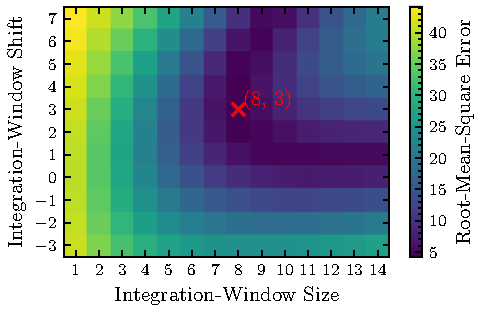
\includegraphics[width=\textwidth]{amp50nsb5}
    \caption{50~p.e. illumination, 5~MHz noise.}
    \label{fig:amp50nsb5}
  \end{subfigure}
  \hfill
  \begin{subfigure}[b]{0.49\textwidth}
    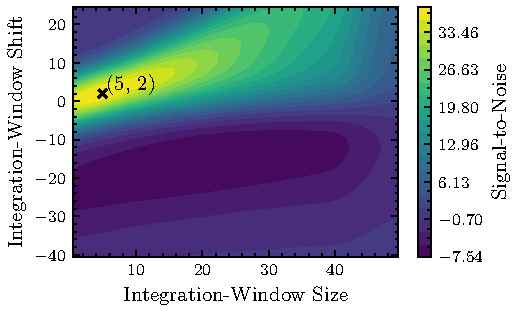
\includegraphics[width=\textwidth]{amp50nsb125}
    \caption{50~p.e. illumination, 125~MHz noise.}
    \label{fig:amp50nsb125}
  \end{subfigure}
  \caption[Optimal integration-window parameters.]{Contour plot of signal-to-noise as a function of window width and shift, for different amplitudes and noise values. The maximum, annotated with the cross and position, indicates the optimal integration-window parameters when applied to a CHEC-S waveform. The contours are split into percentiles of the range; the top \SI{5}{\percent} of values are contained in the brightest yellow contour. Negative values correspond to an integration window concentrated on the undershoot of the pulse.}
  \label{fig:snr_noc}
\end{figure}

As an alternative to the \textit{Cross Correlation} integration approach, one may instead use a simple integration window, defined by the number of samples inside the ``window width'', and the number of samples the window is ``shifted'' from the peak time. The definitions of ``window width'' and ``window shift'' are illustrated in Figure~\ref{fig:charge_extraction_window_wf}. In order to investigate the performance of the integration-window approach fairly, one must first optimise the values for the width and shift of the window when extracting charge from a \gls{chec-s} waveform. This exercise was performed using a Monte Carlo simulation of the lab set-up, where the camera was uniformly illuminated. The pulse time is consistent in simulations of this nature, therefore the same pulse time is manually chosen for every waveform. This allows the following investigation to be solely on the integration approach, avoiding any dependence on the peak finding.

\subsection{Optimal Integration Window Parameters}

As explained in Chapter~\ref{ch6-reduction}, the optimal integration window parameters are noise dependent; a larger integration window is likely to include more noise (\gls{nsb} and \gls{dcr}). However, a larger window size results in more of the signal being captured. In Figure~\ref{fig:snr_noc}, the signal-to-noise ($S/N$) as a function of integration-window parameters is shown for different amplitude and noise values. The $S/N$ investigation was performed as follows. Assume an ``on'' region of the waveform, where the extracted value contains the signal plus the noise, and an ``off'' region where the extracted value contains solely the noise contributions (Figure~\ref{fig:charge_extraction_window_wf}). The optimal window for a constant signal on top of a fluctuating background is then found by:
\begin{equation} \label{eq:snr}
S/N = \frac{\mu_\text{on}}{\sigma_\text{off}},
\end{equation}
where $\mu_\text{on}$ is the average signal extracted from the ``on'' region, and $\sigma_\text{off}$ is the standard deviation of the signal extracted from the ``off'' region. The approach of Equation~\ref{eq:snr} is an alternative to looking for the optimal window for a fluctuating signal on top of a fluctuating background ($S/N = \frac{\mu_\text{on}}{\sigma_\text{on}}$), which, due to the inclusion of the signal deviations from the ``on'' region, is much less sensitive to the noise fluctuations and has a strong dependence on the signal level, i.e.\@ the Poisson fluctuations of the signal increases with amplitude.

In Figure~\ref{fig:snr_noc} the conflict between a large window size to contain the full signal, and a small window to minimise noise is evident, resulting in a limited region in which a high signal-to-noise can be achieved. In conclusion, an integration window width of 5 samples and a shift of 2 samples appeared to be optimal for a noise of \SI{125}{MHz}, for both small and large amplitudes (Figures~\ref{fig:amp1nsb125} and \ref{fig:amp50nsb125} respectively). This integration window is demonstrated in Figure~\ref{fig:charge_extraction_window_wf}. As the \textit{Charge Resolution} requirements are defined at an \gls{nsb} of \SI{125}{MHz}, these window parameters are adopted for the following investigations.

\subsection{Comparison with \textit{Cross Correlation}}

As described previously in the thesis, the most appropriate performance criterion for a charge extraction technique used for a \gls{cta} camera is the \textit{Charge Resolution}. Outlined in Section~\ref{section:crprocedure} are the names I have defined to distinguish between different \textit{Charge Resolution} procedures, each using different datasets and/or procedures. In order to evaluate the performance of the \textit{Cross Correlation} technique with respect to a simple integration window, their resulting \textit{Charge Resolutions} were compared in investigations that explore the relevant parameter space.

\begin{figure}
  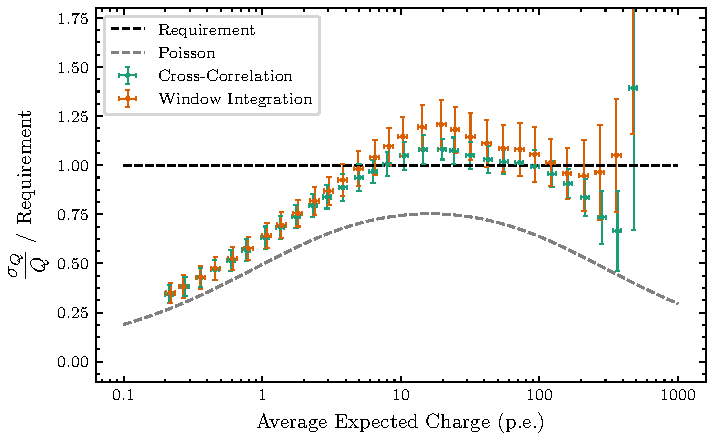
\includegraphics[width=0.9\textwidth]{cr_8_ce_comparison_lab}
  \caption[\textit{Charge Resolution} comparison between \textit{Cross Correlation} and \textit{Window Integration} for \textit{Lab} data.]{\textit{Charge Resolution} of the \textit{Cross Correlation} charge extraction approach applied to uniformly illuminated lab data, compared to the \textit{Charge Resolution} of the integration window approach for the same dataset. The Y axis is limited to exclude the high values that arise from saturation.}
  \label{fig:cr_8_ce_comparison_lab}
\end{figure}

The first comparison is shown in Figure~\ref{fig:cr_8_ce_comparison_lab}. It explores the comparative performance in the context of the measurements using the \textit{Lab} dataset (i.e.\@ using the real camera). A small performance improvement is observed with the cross-correlation technique for $Q_\text{Exp} > 10$~\si{\pe}.

\begin{figure}
  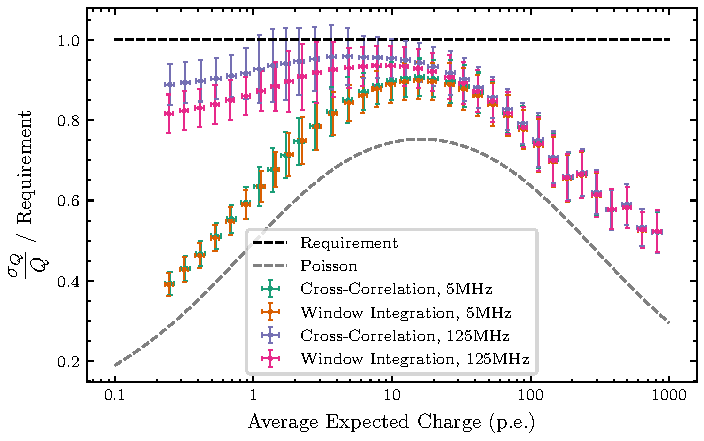
\includegraphics[width=0.9\textwidth]{cr_8_ce_comparison_opct40}
  \caption[\textit{Charge Resolution} comparison between \textit{Cross Correlation} and \textit{Window Integration} for \textit{MCLab} data with an optical crosstalk of \SI{40}{\percent}.]{\textit{Charge Resolution} of the \textit{Cross Correlation} charge extraction approach compared to the \textit{Charge Resolution} of the integration window approach, for both \SI{5}{MHz} and \SI{125}{MHz} \gls{nsb} noise. The dataset used is produced by Monte Carlo simulations of the camera uniformly illuminated, replicating the lab set-up (i.e.\@ the \textit{MCLab} procedure). The optical crosstalk of the photosensors in the simulation is \SI{40}{\percent}.}
  \label{fig:cr_8_ce_comparison_opct40}
\end{figure}

In a comparison of the two extraction approaches when used in a simulation using the \gls{chec-s} model, shown in Figure~\ref{fig:cr_8_ce_comparison_opct40}, it is evident that the \textit{Cross Correlation} approach performs worse than the \textit{Window Integration}, especially at higher \gls{nsb}.

\begin{figure}
  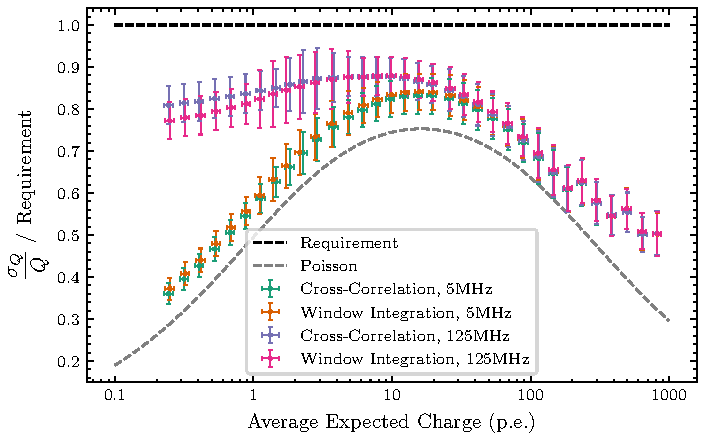
\includegraphics[width=0.9\textwidth]{cr_8_ce_comparison_opct20}
  \caption[\textit{Charge Resolution} comparison between \textit{Cross Correlation} and \textit{Window Integration} for \textit{MCLab} data with an optical crosstalk of \SI{20}{\percent}.]{Same as Figure~\ref{fig:cr_8_ce_comparison_opct40}, but with a dataset containing an optical crosstalk value of \SI{20}{\percent}.}
  \label{fig:cr_8_ce_comparison_opct20}
\end{figure}

Figure~\ref{fig:cr_8_ce_comparison_opct20} shows a similar comparison to the previous one, however the optical crosstalk of the simulation model was reduced to \SI{20}{\percent}. The result is an improved performance when using the \textit{Cross Correlation} technique at low \gls{nsb} rate. However, at high \gls{nsb}, the \textit{Window Integrator} performs slightly better.

\begin{figure}
  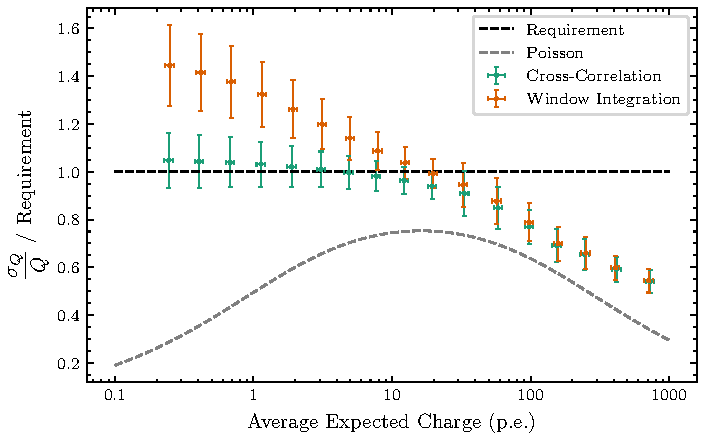
\includegraphics[width=0.9\textwidth]{cr_8_ce_comparison_high_noise}
  \caption[\textit{Charge Resolution} comparison between \textit{Cross Correlation} and \textit{Window Integration} for \textit{MCLab} data with a high amount of electronic noise.]{Same as Figure~\ref{fig:cr_8_ce_comparison_opct40}, but with a dataset containing a factor of 10 higher electronic noise.}
  \label{fig:cr_8_ce_comparison_high_noise}
\end{figure}

Finally, in Figure~\ref{fig:cr_8_ce_comparison_high_noise} a simulation of \gls{chec-s} is used, but with a factor of 10 higher electronic noise. As a result, the \textit{Cross Correlation} technique significantly improves the performance with respect to the \textit{Window Integrator}.

\subsection{Conclusion}

The comparisons of \textit{Charge Resolution} have confirmed our understanding of the \textit{Cross Correlation} method:
\begin{itemize}
\item The \textit{Cross Correlation} method amplifies anything correlated with reference pulse shape. This includes \gls{nsb} and optical crosstalk factors. Therefore, when these are the dominant noise factors in the waveforms, the \textit{Window Integrator} performs slightly better.
\item When noise that is uncorrelated with the reference pulse shape is present in the waveform, such as a high amount of electronic noise, the \textit{Cross Correlation} is an extremely useful tool to resolve the signal.
\end{itemize}
It would appear that with the current simulation model of \gls{chec-s}, the major noise components are those correlated with the reference pulse shape. Therefore, not much improvement is available through the \textit{Cross Correlation} technique. However, when the optical crosstalk of the \glspl{sipmt} is lowered to \SI{10}{\percent} (see Section~\ref{section:sipmt_future}), the other noise factors such as electronic noise could become a relatively significant contribution to the total noise (as occurs in Figure~\ref{fig:cr_8_ce_comparison_opct20}). This would therefore justify the use of the \textit{Cross Correlation} technique. 

Despite the conclusion obtained from the simulations, there does appear to be an improvement when using the \textit{Cross Correlation} method for measurements of the real camera (Figure~\ref{fig:cr_8_ce_comparison_lab}). The only likely source of uncorrelated noise at $Q_\text{Exp} > 10$~\si{\pe} is from the residuals in the Transfer Function calibration. It would appear that the \textit{Cross Correlation} method suppresses this additional noise component introduced by the calibration.  As the Transfer Functions are not present in the simulations, this affect is not apparent in the \textit{Charge Resolution} results obtained from them.

A further investigation into the actual parameter regions of Equation~\ref{eq:charge_res_req} which justify the use of the \textit{Cross Correlation} approach is intended for the future.